\documentclass[]{article}
\usepackage[T1]{fontenc}
\usepackage{lmodern}
\usepackage{amssymb,amsmath}
\usepackage{ifxetex,ifluatex}
\usepackage{fixltx2e} % provides \textsubscript
% use upquote if available, for straight quotes in verbatim environments
\IfFileExists{upquote.sty}{\usepackage{upquote}}{}
\ifnum 0\ifxetex 1\fi\ifluatex 1\fi=0 % if pdftex
  \usepackage[utf8]{inputenc}
\else % if luatex or xelatex
  \ifxetex
    \usepackage{mathspec}
    \usepackage{xltxtra,xunicode}
  \else
    \usepackage{fontspec}
  \fi
  \defaultfontfeatures{Mapping=tex-text,Scale=MatchLowercase}
  \newcommand{\euro}{€}
\fi
% use microtype if available
\IfFileExists{microtype.sty}{\usepackage{microtype}}{}
\usepackage[margin=1in]{geometry}
\usepackage{graphicx}
% Redefine \includegraphics so that, unless explicit options are
% given, the image width will not exceed the width of the page.
% Images get their normal width if they fit onto the page, but
% are scaled down if they would overflow the margins.
\makeatletter
\def\ScaleIfNeeded{%
  \ifdim\Gin@nat@width>\linewidth
    \linewidth
  \else
    \Gin@nat@width
  \fi
}
\makeatother
\let\Oldincludegraphics\includegraphics
{%
 \catcode`\@=11\relax%
 \gdef\includegraphics{\@ifnextchar[{\Oldincludegraphics}{\Oldincludegraphics[width=\ScaleIfNeeded]}}%
}%
\ifxetex
  \usepackage[setpagesize=false, % page size defined by xetex
              unicode=false, % unicode breaks when used with xetex
              xetex]{hyperref}
\else
  \usepackage[unicode=true]{hyperref}
\fi
\hypersetup{breaklinks=true,
            bookmarks=true,
            pdfauthor={Romain Gille \& Yannick Ezvan},
            pdftitle={Analyse des comparaisons des photos},
            colorlinks=true,
            citecolor=blue,
            urlcolor=blue,
            linkcolor=magenta,
            pdfborder={0 0 0}}
\urlstyle{same}  % don't use monospace font for urls
\setlength{\parindent}{0pt}
\setlength{\parskip}{6pt plus 2pt minus 1pt}
\setlength{\emergencystretch}{3em}  % prevent overfull lines
\setcounter{secnumdepth}{0}

\title{Analyse des comparaisons des photos}
\author{Romain Gille \& Yannick Ezvan}
\date{}

\begin{document}
\maketitle

{
\hypersetup{linkcolor=black}
\setcounter{tocdepth}{3}
\tableofcontents
}
\newpage

\section{Photo originale}\label{photo-originale}

\emph{Toutes les comparaisons sont faites avec la photo originale}

\begin{figure}[htbp]
\centering
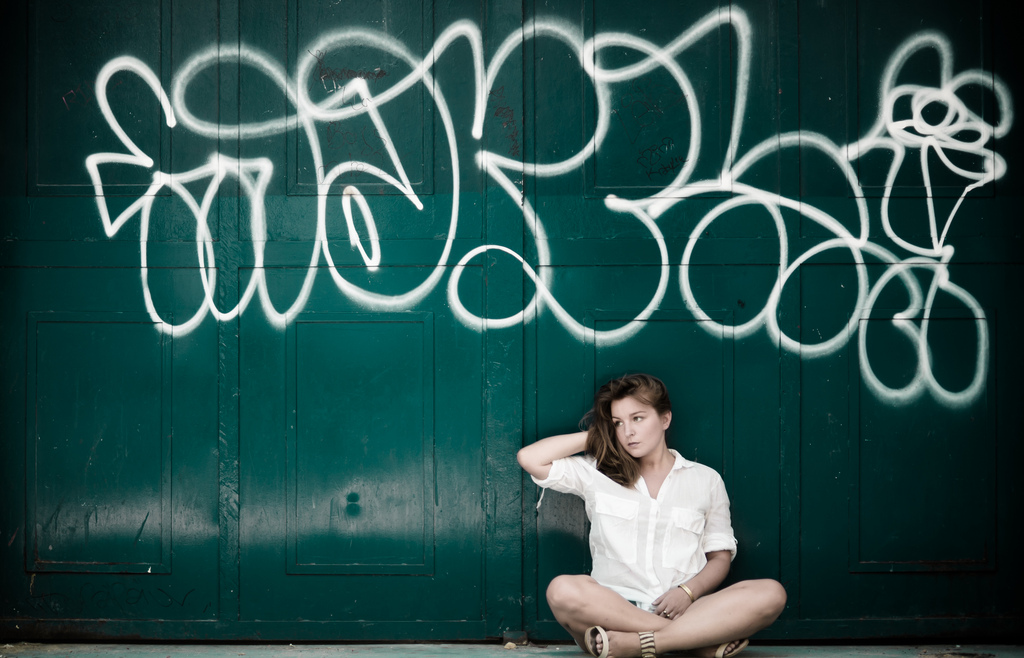
\includegraphics{photos/original.jpg}
\caption{Photo original}
\end{figure}

\newpage

\section{Comparaison avec la photo en contraste
élevé}\label{comparaison-avec-la-photo-en-contraste-uxe9levuxe9}

\begin{figure}[htbp]
\centering
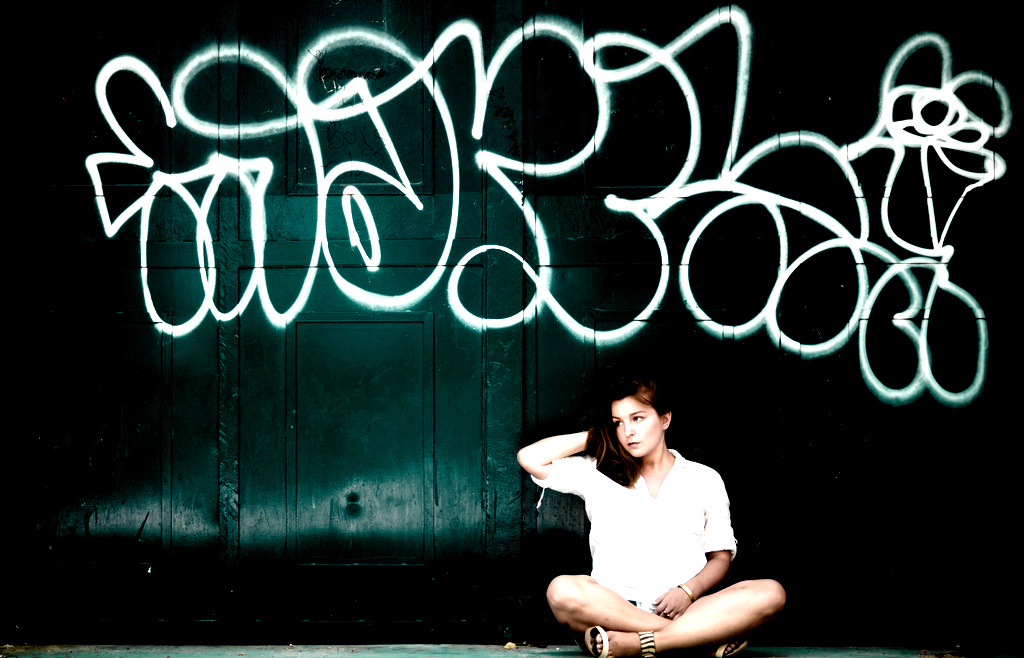
\includegraphics{photos/contraste.jpg}
\caption{Photo contraste}
\end{figure}

On observe que la comparaison de la photo originale avec la photo en
contraste élevée nous donne comme résultat que les deux photos se
ressemblent au niveau de leurs formes mais pas suffisamment d'un point
de vue colorimétrique. Cela s'explique par le fait qu'augmenter les
contrastes d'une photo change ses couleurs et très peu sa forme (on a
relevé seulement $28\%$ de différence par comparaison après
l'application d'un filtre de Sobel contre $35\%$ de différence avec la
distance de Bhattacharyya).

\newpage

\section{Comparaison avec la photo avec un
crop}\label{comparaison-avec-la-photo-avec-un-crop}

\begin{figure}[htbp]
\centering
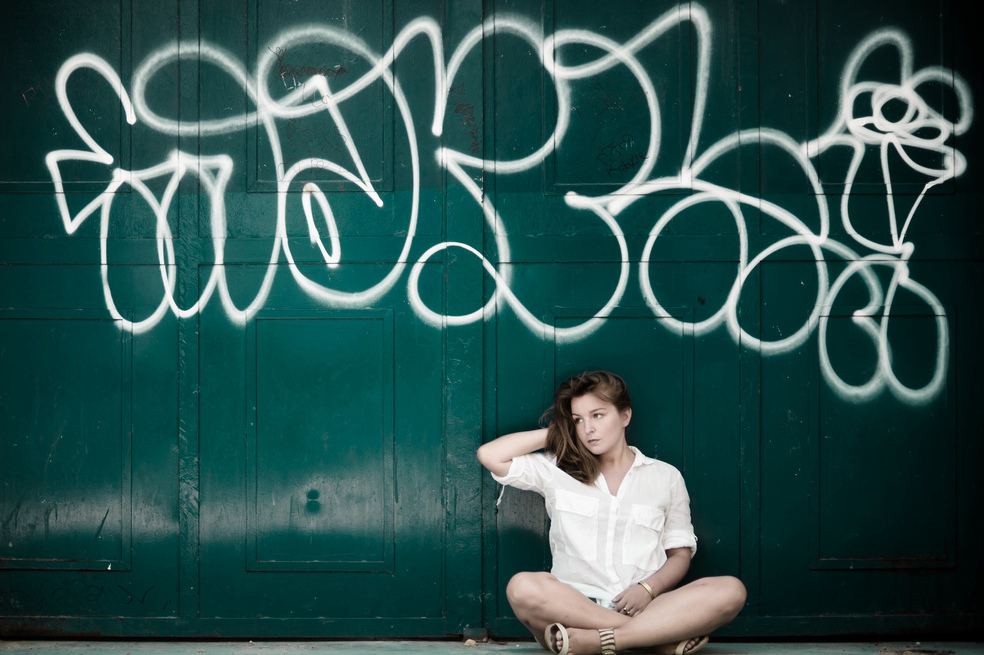
\includegraphics{photos/crop.jpg}
\caption{Photo crop}
\end{figure}

La comparaison de la photo originale avec la photo à laquelle on a
appliqué un crop nous montre une différence très faible au niveau de la
couleur ($0.27\%$ de différence par le filtre de Bhattacharyya) contre
une différenciation prononcée au niveau des formes ($51.16\%$ avec la
comparaison en Sobel). Cela s'explique par le fait qu'un crop est un
redécoupage de la photo et que donc certaines formes délimitables grâce
au filtre de Sobel ne sont plus présentes sur la photo. Cependant les
couleurs ne changent pas ce qui explique ce pourcentage de différence
très faible au niveau colorimétrique.

\newpage

\section{Comparaison avec la photo aux couleurs
inversées}\label{comparaison-avec-la-photo-aux-couleurs-inversuxe9es}

\begin{figure}[htbp]
\centering
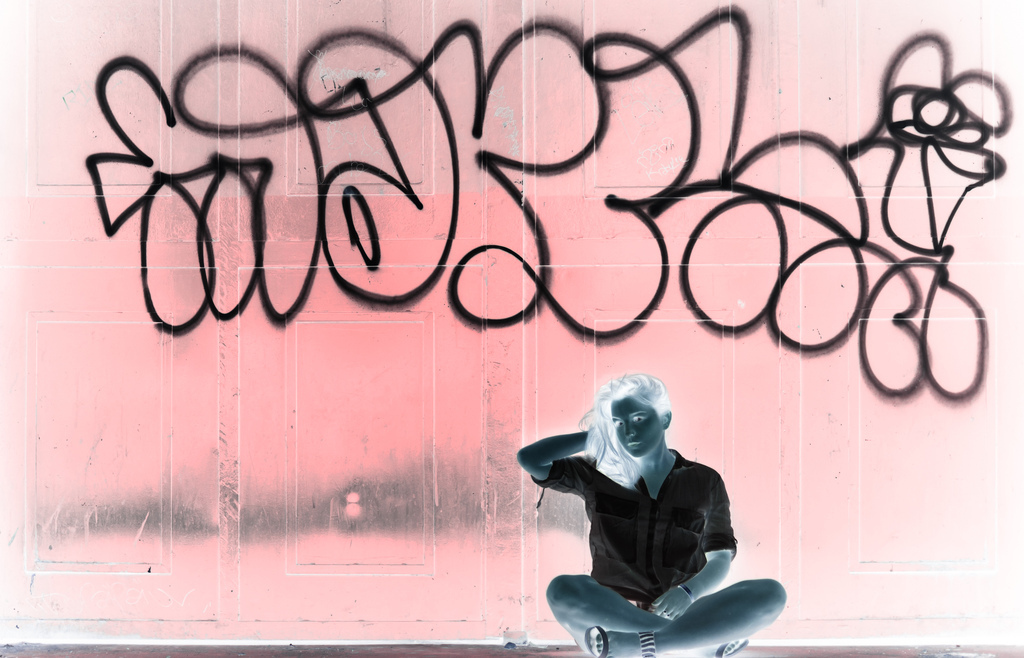
\includegraphics{photos/inverse.jpg}
\caption{Photo couleurs inversées}
\end{figure}

Les résultats de la comparaison de la photo originale avec la photo
inversée nous montre une différence de formes nulle via la comparaison
des photos en Sobel et une différence de $49.49\%$ en distance de
Bhattacharyya. Cela s'explique par le fait que l'inversion des couleurs
ne change pas les formes de la photo.

\newpage

\section{Comparaison avec la photo plus
lumineuse}\label{comparaison-avec-la-photo-plus-lumineuse}

\begin{figure}[htbp]
\centering
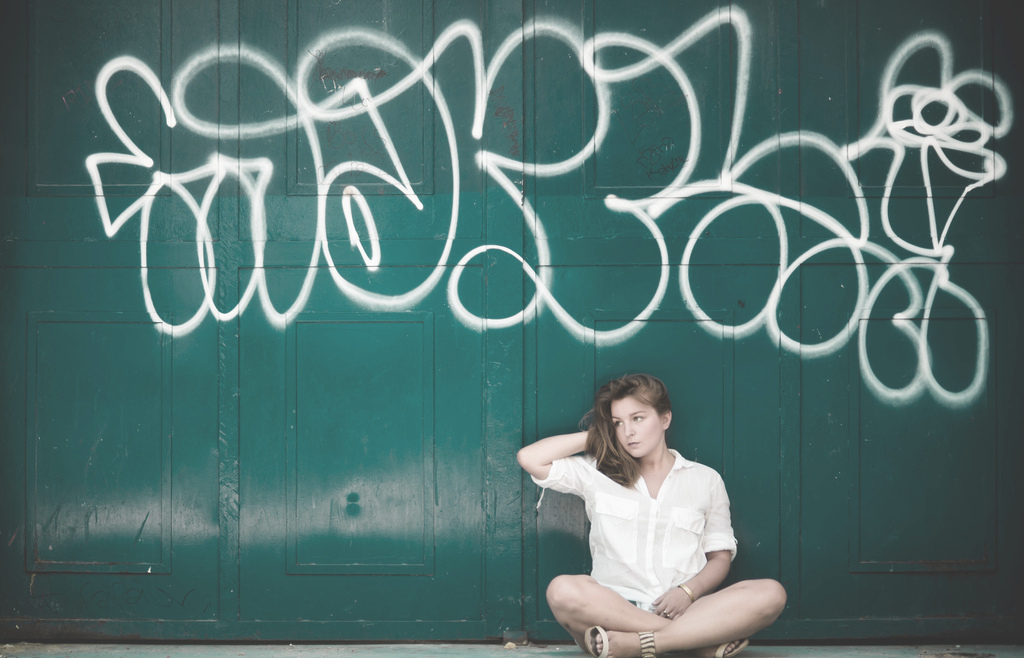
\includegraphics{photos/lumineux.jpg}
\caption{Photo plus lumineuse}
\end{figure}

On observe que la luminosité ajoutée à notre photo d'origine est
suffisante pour donner une différence colorimétrique de $51.53\%$ par la
distance de Bhattacharyya. Par contre, le changement de luminosité ne
change que très peu les contours des formes, seulement $12.43\%$ de
différence après application du filtre de Sobel.

\newpage

\section{Comparaison avec la photo avec effet
poster}\label{comparaison-avec-la-photo-avec-effet-poster}

\begin{figure}[htbp]
\centering
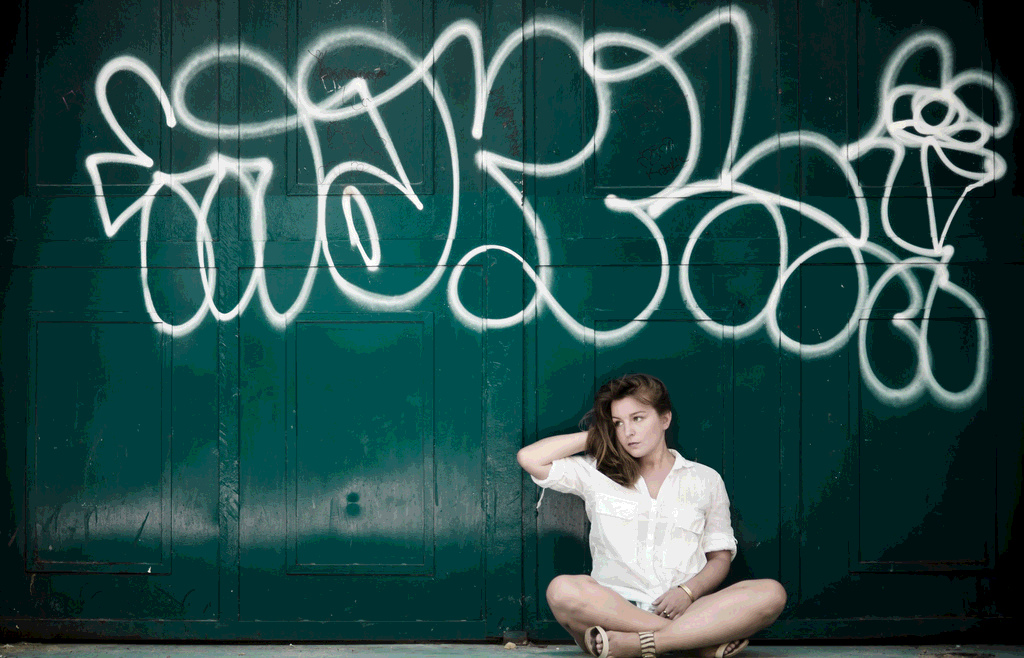
\includegraphics{photos/poster.jpg}
\caption{Photo poster}
\end{figure}

La comparaison de cette image nous donne une différence de $16.35\%$
pour la colorimétrie avec la distance de Bhattacharyya et de $16.79\%$
pour les formes après application du filtre de Sobel. Ce sont des
pourcentages similaires, cependant selon nos critères, la différence
colorimétrique est trop élevée pour dire que les images se ressemblent.
Cependant pour la différence de formes via l'application du filtre de
Sobel, le pourcentage est suffisamment faible pour considérer que les
images se ressemblent d'un point de vue des formes. À l'\oe il nu, on
peut observer que les ombres sont vraiment délimités sur la photo
poster, ce qui explique les $16\%$ de différence trouvés après
application du filtre de Sobel.

\newpage

\section{Comparaison avec la photo avec une légère
rotation}\label{comparaison-avec-la-photo-avec-une-luxe9guxe8re-rotation}

\begin{figure}[htbp]
\centering
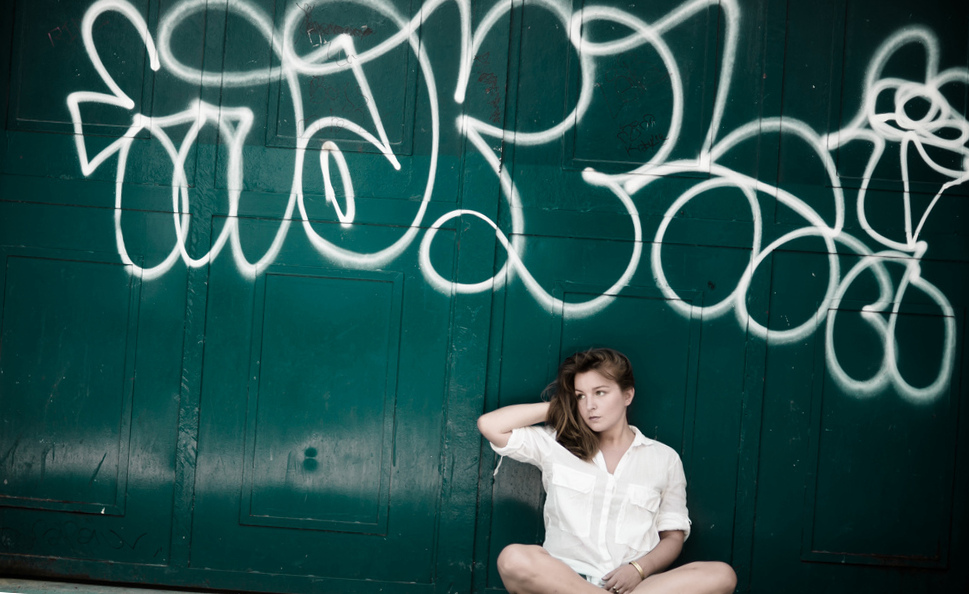
\includegraphics{photos/rotate.jpg}
\caption{Photo rotation légère}
\end{figure}

Pour cette comparaison, on observe une très faible différence de
couleurs (seulement $0.64\%$), car l'image est seulement retournée donc
les couleurs ne changent quasiment pas. Par contre la différence de
formes est assez élevée car tous les pixels sont décalés ($53.58\%$ de
différence après application du filtre de Sobel).\\On constate donc que
la rotation légère ne change pas beaucoup les couleurs de la photo mais
majoritairement ses formes.

\newpage

\section{Comparaison avec la photo d'une rotation de
$90^{\circ}$}\label{comparaison-avec-la-photo-dune-rotation-de-90circ}

\begin{figure}[htbp]
\centering
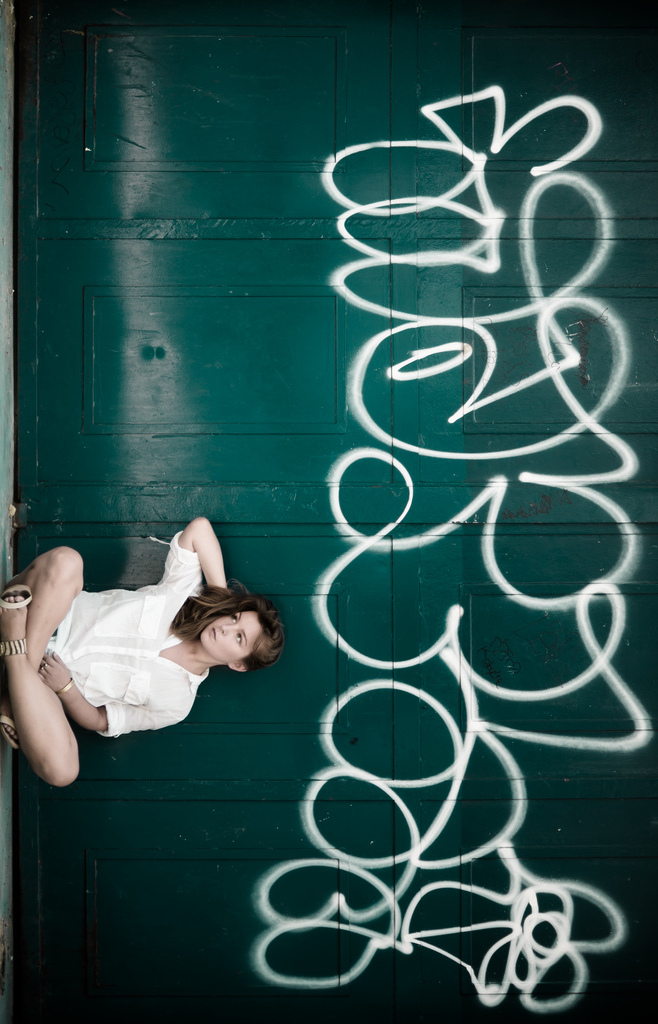
\includegraphics[scale=0.47]{photos/rotation.jpg}
\caption{Photo rotation $90^{\circ}$}
\end{figure}

Contrairement à la photo précédente, cette rotation de $90^{\circ}$ ne
découpe pas l'image donc la différence de couleur est encore plus faible
($0.04\%$) alors que la différence de forme augmente encore ($58.03\%$).

\newpage

\section{Comparaison avec la photo en saturation plus
élevée}\label{comparaison-avec-la-photo-en-saturation-plus-uxe9levuxe9e}

\begin{figure}[htbp]
\centering
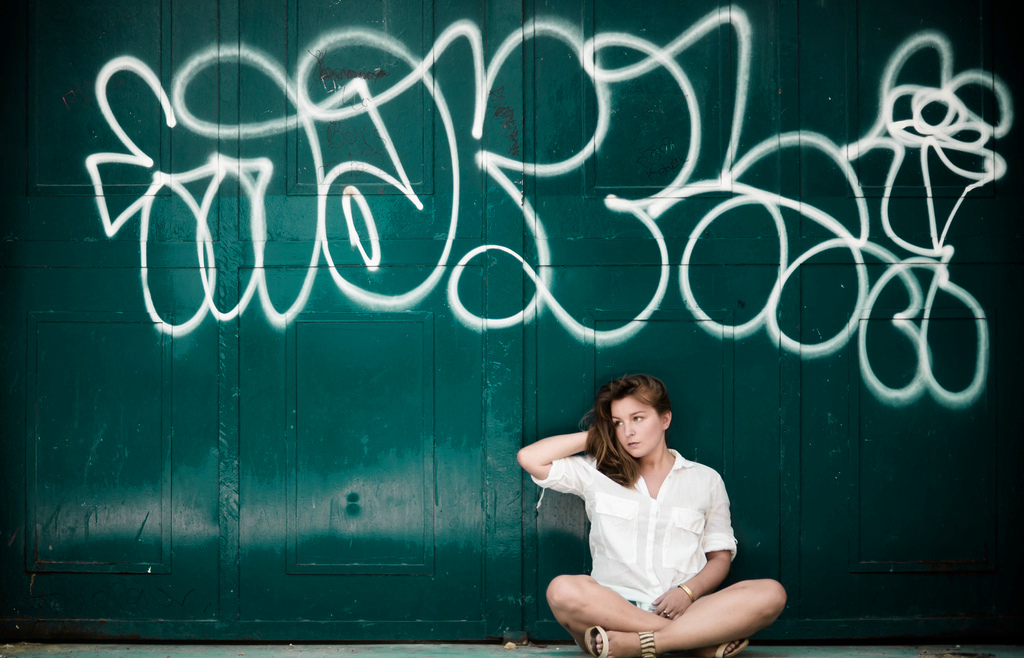
\includegraphics{photos/saturate.jpg}
\caption{Photo en saturation élevée}
\end{figure}

On observe avec la comparaison de cette photo saturée que selon nos
critères, ces deux photos se ressemblent ($0.94\%$ de différence pour la
colorimétrie avec la distance de Bhattacharyya et $0.51\%$ de différence
pour les formes avec l'application du filtre de Sobel).\\En effet, les
couleurs sont légèrement moins ternes sur la photo saturée et les
quelques contours décelés au filtre de Sobel sont dû aux points de
lumière qui sont plus visibles et détourés.

\newpage

\section{Comparaison avec la photo
assombrie}\label{comparaison-avec-la-photo-assombrie}

\begin{figure}[htbp]
\centering
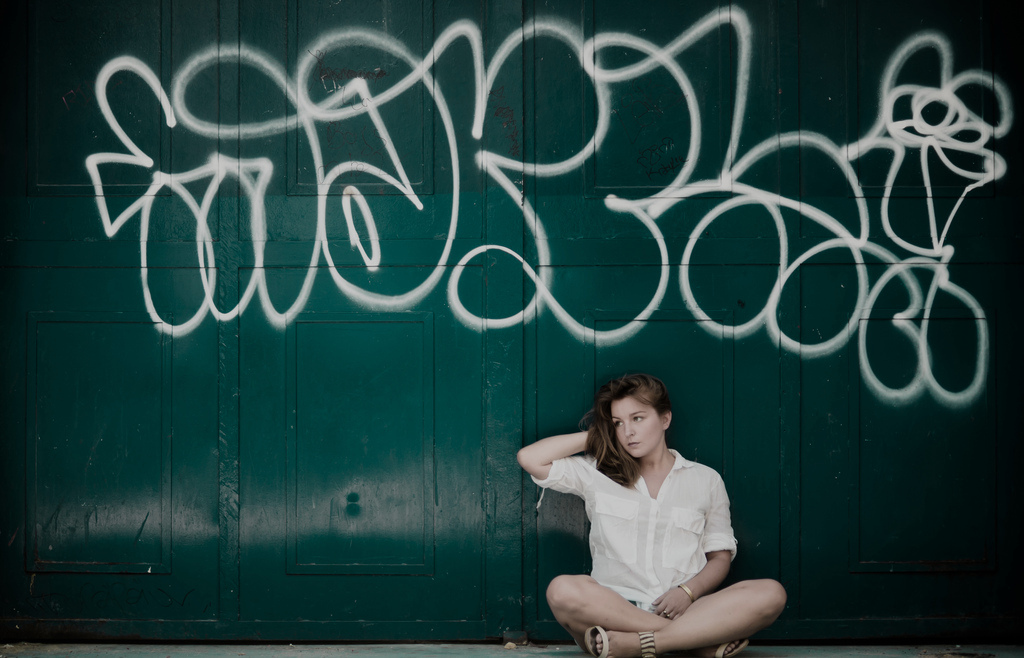
\includegraphics{photos/sombre.jpg}
\caption{Photo sombre}
\end{figure}

Comme pour la photo précédente, on peut considérer que les deux photos
se ressemblent, cependant elles n'ont pas le même niveau de
ressemblance. En effet celle-ci à une différence de $6.44\%$ pour la
colorimétrie par distance de Bhattacharyya et de $12.6\%$ pour les
formes avec le filtre de Sobel. On peut donc conclure que
l'assombrissement de la photo n'a qu'un faible impact sur la photo aussi
bien d'un point de vue de la couleur que des formes.

\newpage

\section{Comparaison avec la photo
terne}\label{comparaison-avec-la-photo-terne}

\begin{figure}[htbp]
\centering
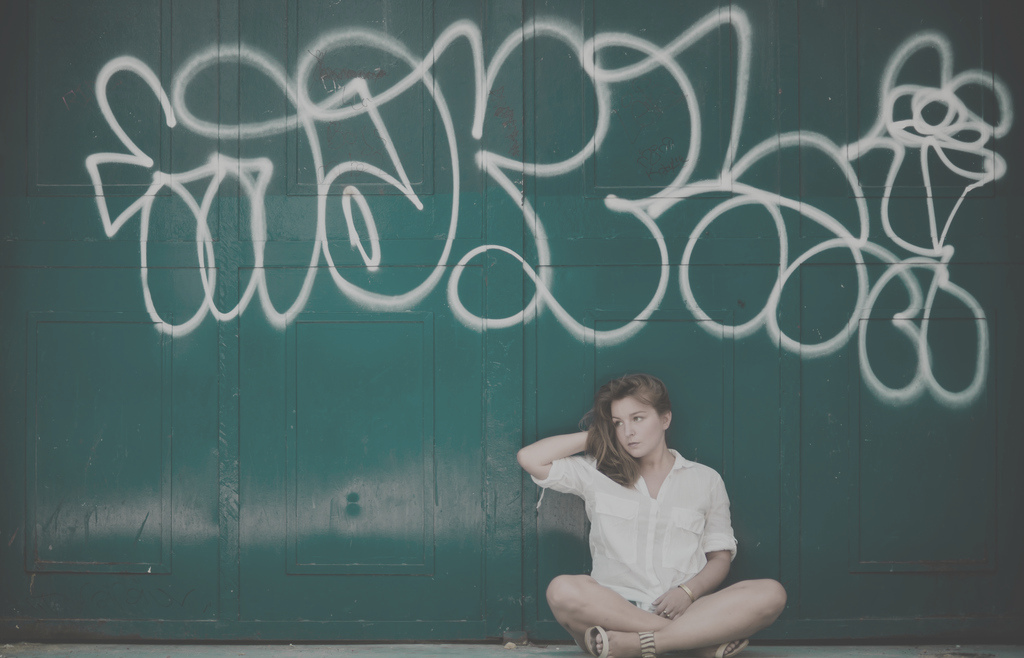
\includegraphics{photos/terne.jpg}
\caption{Photo terne}
\end{figure}

Cette modification a un gros impact sur la photo originale, surtout au
niveau des couleurs. On observe en effet $71.67\%$ de différence au
niveau colorimétrique et $27.33\%$ de différence au niveau des formes.
On peut observer sur la photo directement que toutes les couleurs ont
changées ce qui explique les $71\%$. Les $27\%$ des formes sont dues aux
bordures que ce filtre doit atténuer.

\end{document}
